% $File: report.tex
% $Date: Sat Oct 19 14:34:59 2013 +0800
% $Author: wyx <ppwwyyxxc@gmail.com>

\documentclass[11pt,a4paper]{article}
\usepackage{threeparttable}
\usepackage{dirtree}
\usepackage{keystroke}


\usepackage{fontspec,amsmath,amssymb,zhspacing,verbatim,minted,listings,zhmath}
\usepackage{titlesec, titletoc}
\usepackage{enumerate}
\usepackage[hyperfootnotes=false,colorlinks,linkcolor=blue,anchorcolor=blue,citecolor=blue]{hyperref}
\usepackage[backend=biber]{biblatex}
%\usepackage[dvips]{graphicx}
\usepackage{subfigure}
\usepackage{indentfirst}
\usepackage{float}			% don't automatically change location of figure [H]
\usepackage{chngpage}		% use \changetext to change page size
\usepackage{caption}\captionsetup{hypcap=true}  % ref to jump to object instead of caption
\newfontfamily\zhfont[BoldFont=SimHei,ItalicFont=KaiTi_GB2312]{SimSun}
\lstset{keywordstyle=\color{blue!70}, commentstyle=\color{red!50!green!50!blue!50},frame=shadowbox,rulesepcolor=\color{red!20!green!20!blue!20},
basicstyle=\footnotesize\ttfamily}
\zhspacing
\setlength{\parindent}{2em}

\usepackage{fancyhdr}
\changetext{}{2.2cm}{-1.1cm}{-1.1cm}{}
\pagestyle{fancy}
\setlength{\headheight}{15.2pt}
\lhead[]{}\rhead[]{}
\fancyhead[C]{\emph{Uknow InfoHub}}


%use cell in tabular
\newcommand{\tabincell}[2]{\begin{tabular}{@{}#1@{}}#2\end{tabular}}

%thick shline
\newlength\savewidth
\newcommand\shline{\noalign{\global\savewidth\arrayrulewidth\global\arrayrulewidth 1pt}
                   \hline
                   \noalign{\global\arrayrulewidth\savewidth}}


\defbibheading{bibliography}{\section{References}}
\bibliography{refs.bib}
\newcommand{\figref}[1]{\hyperref[fig:#1]{Fig. \ref*{fig:#1}}}
\newcommand{\secref}[1]{\hyperref[sec:#1]{Sec. \ref*{sec:#1}}}
\newcommand{\tabref}[1]{\hyperref[tab:#1]{Tab. \ref*{tab:#1}}}

% math function
\let\Oldsum\sum
\renewcommand{\sum}{\displaystyle\Oldsum}
\let\Oldprod\prod
\renewcommand{\prod}{\displaystyle\Oldprod}


../mint-defs.tex

\title{Uknow InfoHub \\ \small Production Requirement Documentation}
\author{BlXLRSMB Team}
\date{}

\begin{document}

\titleformat*{\section}{\centering\Large\bf}
\setlength{\baselineskip}{1.3em}
\fontsize{13}{\baselineskip}\selectfont


\maketitle
\tableofcontents

\newcolumntype{L}{>{\centering\arraybackslash}m{3cm}}

\section{Introduction}
\label{sec:intro}
\subsection{Document Introduction}
\label{sec:introduction}
	In the following sections of this document, we will present several skim of our project management.

	In~\secref{git}, how we use git as the subversion tool. Issues and milestones will be presented in~\secref{issue}.



\section{Functional Requirement}
%File: functional-user.tex
%Date: Sat Oct 19 13:43:10 2013 +0800
%Author: Yuxin Wu <ppwwyyxxc@gmail.com>

\subsection{User Management}

An user's permitted behaviors on his/her account are included in but not
limited to the following:

\begin{itemize}
\itemsep1pt\parskip0pt\parsep0pt
\item
  Register an account
\item
  Login
\item
  Edit his/her personal profile
\item
  Change his/her password
\item
  Delete his/her account, along with all the data the user has provided
  to Uknow.
\end{itemize}

%File: functional-data.tex
%Date: Sat Oct 19 14:12:08 2013 +0800
%Author: Xinyu Zhou <zxytim@gmail.com>

\subsection{Data Management}

\subsubsection{Items}

An item is piece of information retrieved from various sources, and
shown in lists for further reading. It consists of following parts:

\begin{itemize}
\itemsep1pt\parskip0pt\parsep0pt
\item
  Title
\item
  Source
\item
  Content
\item
  Labels
\item
  Comments
\end{itemize}

Item is the core entity in Uknow system. A user can manipulate items in
following ways:

\begin{description}
\item[Removal] \hfill

  When a user find a specific item unpleasant, unattractive or redundant, he/she
  may remove this item using the button provided. Removal operation can be
  reversed within a short period of time to prevent from mis-clicking the button.

\item[Archive] \hfill

  User can store specific items for further reading or recapping in
  the future. Archived items still show up in item flow, and will be
  labeled as `archived'.

\item[Share] \hfill

  If an item fascinates a user, he/she may share it among popular SNS.
  When first sharing an item, user will authenticate its account on
  desired SNS website, and after confirmation, a sharing information
  will be posted on the chosen SNS.

\item[Like] \hfill

  Users can show theirs preferences on certain items, and others will
  know the statistics, and this could be used as an score to evaluate an
  item. For a better reading experience, high score items are more likely to rank higher in the item flow than low score items.

\item[Comment] \hfill

  Users can post comments under an item. Posts will be stored in
  this system, and can optionally be posted synchronously on item
  source, if the source website supports such functionality.

  Comments is organized hierarchically. If a user intends to reply
  other's comment, he/she can click the reply button, and the
  reply form should show right below the comment.

  When complete typing, click the reply button and the comments shall be
  posted, and the form will consequently disappear.
\end{description}

Furthermore, system can learn from user behaviors on items and to
recommend items related to users' interest.

\subsubsection{Labels}

A label is an attribute describing items. An item can have multiple
labels. A label associated with an item may be automatically assigned by
system, or tagged by users. A label can be either a system-wide label,
which is visible to all user, or a user specified label which indicates
user preferences on an item.

Label may come from:

\begin{description}
\item[System Pre-tagging]
  An item may arrive to a user with pre-tagged
  labels. These pre-tagged labels are vital to subsequent data
  processing, such as tag-filtering plugins in tabs.

\item[User-tagging]
  Same item could have distinct meaning to different user.
  User can tag item with labels cater to their taste, as well as remove
  labels that could lead to misunderstanding to itself.
\end{description}

As described aforementioned, functions like `archive' is actually a process of tagging an
item by the label `archived'

\subsubsection{Plugins}

Plugin is an essential concept in Uknow system, which comprises the
implementations of varied functionalities in the system. A plugin should
process a bunch of items, returning processed items. The number of items
before and after need not to be the same, that is, a plugin can either
shrink items or enrich items (filtering job) or process on contents of
items.

User can choose a subset of provided plugins to employ on its items.
Plugin can be either scoped to a `tab' or can be applied system-wide.

Plugins can be configurable, but configuration is plugin-dependent.

Examples of plugins:

\begin{description}
\item[Tag-filtering] Allowing users to choose preferred tags.
\item[Highlight] Highlight significant words in an item.
\item[Emotion tagging] Detect emotion of an item.
\item[Face detection in image] Detect faces from images of an item.
\item[Related items] Recommend related items for users to discover new contents to read.
\end{description}

\subsubsection{Tabs}

Tab is a collection of filtered items, in which the filter is defined by
plugins. A typical use of tab is to divide items into different
categories, which can be exclusive or not.

Tabs can be added or removed on-the-fly with `add' or `remove' button,
add define its behaviour with plugins.

Moreover, tab layout, item flow style, etc., are also configurable via
tab configuration.



%File: non-functional.tex
%Date: Sat Oct 19 22:37:37 2013 +0800
%Author: Yuxin Wu <ppwwyyxxc@gmail.com>

\section{Non-functional Requirements}
%File: non-functional-user.tex
%Date: Sat Oct 19 17:06:09 2013 +0800
%Author: Yuxin Wu <ppwwyyxxc@gmail.com>

\subsection{User Management}

\subsubsection{Register Page}

The register page contains an input form, users can only successfully
register an account if:

\begin{itemize}
\itemsep1pt\parskip0pt\parsep0pt
\item
  The username is unique in our database, and contains only letters and
  digits.
\item
  The password is no less than 6 characters, and does not contains
  digits only.
\item
  User repeat the password again correctly.
\item
  User provided a valid email address.
\end{itemize}

After a valid register form is submitted, the server side would again
check the input values. If the form passes, a validation email would
automaticlly be sent to the user with a confirm code. Otherwise, the
client will redirect the user to the original register page again, and
alert about this error message. This process is illustrated well in \figref{register}.

\begin{figure}[H]
  \centering
  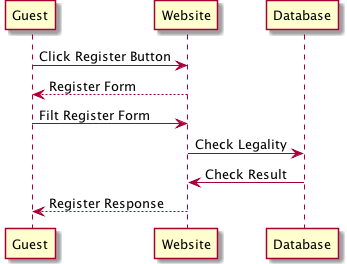
\includegraphics[width=0.6\textwidth]{img/register.png}
  \caption{Registration process\label{fig:register}}
\end{figure}


\subsubsection{Confirm Page}

A link to the confirm page should be attached in the email sent to the
user. An user account will be activated only if:

\begin{itemize}
\itemsep1pt\parskip0pt\parsep0pt
\item
  The email address was registered before but has not been activated
  yet.
\item
  User visits the confirm page within the time constraints.
\item
  A correct confirm code (dependent on this account only) is provided by
  the user.
\end{itemize}

Once an account is activated, user can then edit profile, change
password, and use all the other services provided by Uknow.

\subsubsection{Login/Logout Page}

A visitor will be redirected to login page everytime he/she tries to
visit a restricted resource. In the login page, the user is asked to
provide username together with password. A session is stored in cookie
after a successful login, otherwise, a ``password error'' message will
be displayed. On logging out, this session shall be destroyed and user will be
redirected to the  home page.
The login/logout process is illustrated in \figref{login} and \figref{logout}.
\begin{figure}
\begin{minipage}[b]{0.57\linewidth}
  \centering
  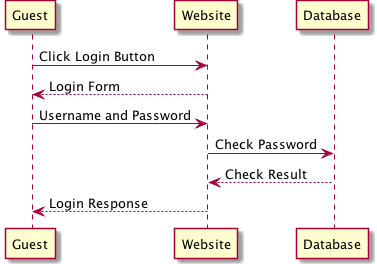
\includegraphics[width=\textwidth]{img/login.png}
  \caption{Login Process \label{fig:login}}
\end{minipage}
\begin{minipage}[b]{0.37\linewidth}
  \centering
  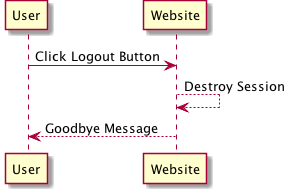
\includegraphics[width=\textwidth]{img/logout.png}
  \caption{Logout Process \label{fig:logout}}
\end{minipage}
\end{figure}



\subsubsection{Profile Page}

User can view and edit the following items:

\begin{itemize}
\itemsep1pt\parskip0pt\parsep0pt
\item
  Avatar, this could be uploaded by user or selected from Gravatar.com
\item
  Nickname, which is displayed in the front page of the site.
\item
  Sex, you know what I mean.
\item
  Age, those under 16 is supposed to be warned before accessing items
  with specific labels.
\item
  Email address, another validation email will be sent if this item is
  changed
\end{itemize}

On the other hand, users should be able to provide access to some social
networking sites for us to collect information including but not limited
to:

\begin{itemize}
\itemsep1pt\parskip0pt\parsep0pt
\item
  Weibo, a twitter-like site in mainland China.
\item
  Renren, a facebook-like site which is very popular among Chinese
  students
\item
  QQ, a MSN-like IM tool running by Tencent
\item
  Tsinghua Netclass, specially provided for Tsinghua student
\end{itemize}

Finally, if user wishes to delete his/her account, a confirm email will
also be sent.

\subsubsection{Change Password}

The password of an account could be changed only if:

\begin{itemize}
\itemsep1pt\parskip0pt\parsep0pt
\item
  The correct old password is provided
\item
  A new valid password.
\item
  The new valid password is typed twice and matched well.
\item
  The link to a confirm page which was emailed to the user was clicked
  within 24h.
\end{itemize}


\subsection{Data Flow and Internal Logic}

The back-end of Uknow InfoHub system comprises mainly five components: item
fetcher, prefilter, data storage, postfilter and API website, as
illustrated in \figref{architecture}.
Data passing between modules are encoded using json formats.

\begin{figure}[H]
  \centering
  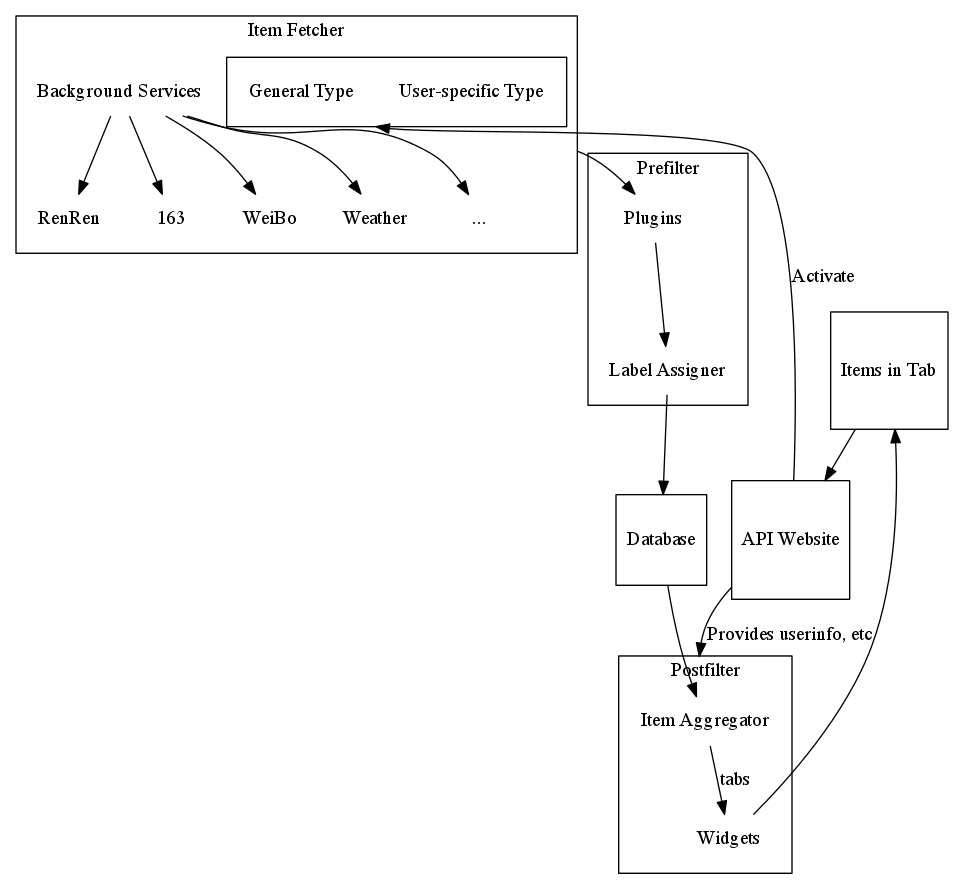
\includegraphics[width=\textwidth]{img/architecture.png}
  \caption{Overall architecture of Uknow backend\label{fig:architecture}}
\end{figure}


\subsubsection{Item}

An item is an abstract concept standing for a piece of collected
information to be presented to the user. It can be almost anything, such
as a status on SNS like renren, a piece of news from Netease, or a Weibo post
or tweets. An item is represented as a dictionary structure
programmatically. Following attributes are associated with an item:

\begin{enumerate}
\def\labelenumi{\arabic{enumi}.}
\itemsep1pt\parskip0pt\parsep0pt
\item
  An integer unique ID, which is used system-widely to identify a
  specific item.
\item
  Item fetcher type, which could be general item fetcher or a
  user-specific item fetcher along with the user ID. See descriptions
  below for further details.
\item
  A set of labels, each of which describes a property of the underlying
  item. Possible labels include data source (websites such as renren,
  Facebook), data category (news, SNS updates, and etc.), and inferred
  information such as its importance to the user. An item could either
  be public or user-specific, and the associated labels could be
  different for different users.
\item
  A description generated by ItemDesc classes, which could be used to render
  HTML entry, for plugins involving NLP(nature language processing), or for item
  searching.
\item
  Creation time
\item
  Other attributes for a specific item category.
\end{enumerate}

\subsubsection{Item fetcher}

\begin{figure}[H]
  \centering
  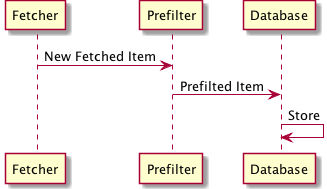
\includegraphics[width=0.6\textwidth]{img/fetch.png}
  \caption{Workflow of Fetcher \label{fig:fetcher}}
\end{figure}


Item fetchers simply retrieve items from various information sources,
adding basic attributes such as ID, description, source URL (if
available), and then forward items to prefilter for later processing, as illustrated in \figref{fetcher}.
There are two types of item fetcher:

\begin{description}
\item[General Item Fetcher]\hfill

  This kind of item fetcher collects public
 such as news and weather. They should always run in
  background and provide new data. No user login or authentication
  should be involved at this stage.
\item[User-specific Item Fetcher] \hfill

  This kind of item fetcher is activated by
  user action (such as login); when activated, it would collect
  information that could only be gained after authentication (such as
  connecting to SNS sites). The API website sends an activation signal
  along with corresponding user ID to all this kind of item fetchers,
  and they should do the work in background. Note that the activating
  process is asynchronous and the user could only get results of some
  time earlier to his request; however the latency should be fairly
  small if fast servers and Internet connection are guaranteed.
\end{description}

\subsubsection{Prefilter}

Prefilter is responsible for processing an item before putting it into
database. Prefilter consists of a series of plugins, each of which takes
the item dictionary as input and outputs a possibly modified item or
aborts processing of current item and discards it. This series comprises
two parts configured by the system administrator and the users
respectively. For the system-wide part, common plugins include infer
extra labels from item content or filtering illegal items. For items
produced by a user-specific item fetcher, plugins enabled by the
corresponding user is referred to as the ``user part'' and would be
applied on this item.

\subsubsection{Database Storage}

After processed by prefilter, if an item is not discarded, it would be
stored in the database. Due to the heterogeneous nature of data items,
we decided to use MongoDB as the storage back-end. The advantages would
be discussed later in \secref{data}.

\subsubsection{Postfilter}

Postfilter contains two stages:

\begin{enumerate}
\def\labelenumi{\arabic{enumi}.}
\itemsep1pt\parskip0pt\parsep0pt
\item
  Item Aggregator: When a user requests items in a tab, possibly with
  time, page number or seaching keyword constraints, the item aggratator
  simply finds items meeting those conditions and return them in some
  order.
\item
  Like prefilter, a sequence of system-wide and user-defined plugins are
  then applied to the items, which, for example, could deduplicate items
  in the same tab.
\end{enumerate}

\subsubsection{API Website}

\begin{figure}[H]
  \centering
  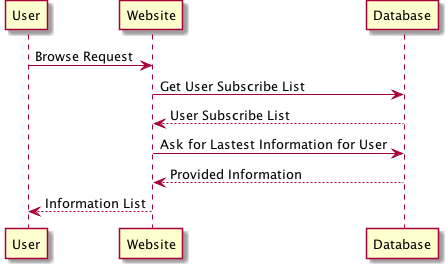
\includegraphics[width=0.6\textwidth]{img/browse.png}
  \caption{Workflow of the API website\label{fig:website}}
\end{figure}


API Website is the interface of the back-end system which interacts with
users, though indirectly. It accepts user requests, invokes
corresponding functions as described above, fetches and presents result
back to user, as displayed in \figref{website}. Refer to \secref{webapi} for further discussion about the API interfaces.

\subsection{Scalability}

\subsubsection{Data Storage}
\label{sec:data}
Data storage is implemented using MongoDB\footnote{\url{http://www.mongodb.org/}},
which is a leading NoSQL databse proven to be fast, stable, flexible and reliable.
Care has to be taken on creating
appropriate indexes to allow fast querying. Techniques such as
replication and sharding could be adopted to enhance efficiency and
reliability, only if there are enough servers. With the help of such
mature production, we do not have to worry too much about data storage.

\subsubsection{Background Workers}

As mentioned above, there are long running background workers fetching
items from public information sources. As the total number of such
sources is limited, it is not necessary to deploy many of those workers, and this
obviously has no scalability issue with growth of user group.

However, user-specific fetchers must be able to scale with the number of
users. Here we set up a worker cluster. The cluster contains a task
queue and distributed worker nodes. When a user activates a fetcher, a
task is added to the queue, and some worker node then picks up the task
and finishes it asynchronously. We choose
Celery\footnote{\url{http://www.celeryproject.org/}}, a distributed, asynchronous task queue to be the queue framework in Uknow.
For a worker node, it must be equipped with high-speed Internet
connection; and we can use co-routines (e.g., greenlet\footnote{\url{https://pypi.python.org/pypi/greenlet}} in Python)
to reduce CPU workload.

Now the system is fully horizontally scalable; theoretically a large
number of users could be served simultaneously if sufficiently many
servers are available.

\subsection{Availablity}

The key to increasing availability is to introduce redundancy. There
could be multiple queue schedulers and multiple worker nodes, failure of
any of which would not influence the whole system. The replication
mechanism provided by MongoDB also guaranteed the availability of data
storage. For API website, we could set up an Nginx\footnote{\url{http://wiki.nginx.org/Main}} server with reverse
proxy to multiple API servers, which makes the whole system almost as
reliable as anyone would request.

\subsection{Security}

The python drivers for MongoDB makes it impossible to commit attacks like SQL
injection. It is hard for our system itself to contain any security
vulnerabilities. Care has to be taken on system security such as server
software, operating system configuration and etc.



\subsection{Web API}

\label{sec:webapi}
Since we provide several different clients, the communication between
client and server should be universal. Thus, web API implemented in Python and based on JSON will
be used.

JSON (JavaScript Object Notation)\footnote{\url{http://www.json.org/}} is a lightweight data-interchange
format. It is easy for humans to read and write. It is easy for machines
to parse and generate. It is based on a subset of the JavaScript
Programming Language, Standard ECMA-262 3rd Edition - December 1999\footnote{\url{http://www.ecma-international.org/publications/files/ecma-st/ECMA-262.pdf}}.

\subsubsection{Basic Structure}

All returned valued is a dict containing some specific keys. If an error
occurred during an API access, a key named \texttt{error} will be
provided with a key named \texttt{msg} showing the reason of error.
Otherwise, the desired data will be returned.

\subsubsection{User Management}

All user management related action should be accessible by API including
but not limited to:

\begin{itemize}
\itemsep1pt\parskip0pt\parsep0pt
\item
  Register an account
\item
  User login (validate)
\item
  Edit profile
\item Withdraw authority for specific third-party web service
\item
  Delete an account
\end{itemize}

When a password is sent, SSL/TLS protocal should be used.

\subsubsection{Data Flow}
Any client of Uknow shall follow an uniformed protocal to commuticate data with Uknow backend server.
Thus, Uknow server shall provide web API for clients to fetch feeds data, mainly consisting of the following parts:
\begin{enumerate}
  \item Get new feeds
  \item Tag an item
  \item Update tab configurations
  \item Update tab-level plugins
\end{enumerate}





\section{Documentation Requirements}

\subsection{License}

\subsubsection{Registration License}

In order to provide better service to our users, users shall claim to
agree our registration license when applying for an account. The
registration license shall cover the following parts:

\begin{enumerate}
\def\labelenumi{\arabic{enumi}.}
\item
  Rules on using our service, including the constrains on using,
  transfering the account, the limited use of the information we
  provided.
\item
  The privacy on the personal information provided by users in
  registration.
\item
  User shall understand and accept the service provided by Uknow before
  registration, and take full responsibilities for any kind of abuse of
  our service.
\end{enumerate}

\subsubsection{Disclaimers}

In order to avoid unnecessary conflicts with our users, users must sign
our disclaimers before using the information collector of Uknow InfoHub.
The disclaimer shall cover the following contents:

\begin{enumerate}
\def\labelenumi{\arabic{enumi}.}
\item
  Uknow is not responsible for, and expressly disclaims all liability
  for, damages of any kind arising out of use, reference to, or reliance
  on any information provided by Uknow.
\item
  While the information provided by Ukonw is periodically updated, no
  guarantee is given that the information is correct, complete, and
  up-to-date.
\item
  Though Uknow might provide links or direct data from other Internet
  Resources, Uknow is not responsible for any kind of damages arising
  out of visit to those sites.
\item
  Uknow doesn't own and shall not preserve copyright for any information
  provided in our service, but will show the user the origin of those
  information. Any kind of offence to the copyright of the original
  author of the information provided by us is seen as a direct offence
  to the author.
\item
  Though Uknow might contain advertisements or other types of
  endorsement for products or services from third-party companies, Uknow
  has not investigated and does not assure the fidelity of the claims by
  any advertiser. Product information is based solely on material
  received from suppliers.
\end{enumerate}

\subsubsection{Notice to Right Holders}

Uknow InfoHub developer group understand and respect the right of any
individual or entity. Thus, a notice to right holders must be provided
on our website for right holders to read and get instructions on
enforcement of their corresponding rights related to the behavior or the
services provided by Uknow InfoHub developer group. The notice shall
cover the following parts:

\begin{enumerate}
\def\labelenumi{\arabic{enumi}.}
\item
  Copyright. While Uknow InfoHub provides simple information aggregation
  for our terminal users, Uknow respects and does not offend the
  copyright of the original author of the information presented by us.
\item
  Privacy. Uknow might fetch and parse information from various sources,
  but with the authority of our service users. Uknow will not
  initiatively collect private data of any individual or entity.
\item
  Use of our service. All users of our services are immediately granted
  the right of using our service according to the user agreement right
  after registration.
\end{enumerate}

\subsection{Help Manual}

\subsubsection{Basic Use of Our Service}

For the purpose of getting users quickly involved in our product, an
instruction manual on the basic use of our service is necessary. This
instruction manual shall contain the following parts:

\begin{enumerate}
\def\labelenumi{\arabic{enumi}.}
\item
  The functionality of our service, and the instructions of using them
  on our clients.
\item
  Examples on the use of our key functionality, including tab-like
  information classification, auto-tagging, etc.
\item
  Precautions and attentions that our users should be aware of.
\end{enumerate}

\subsubsection{API Documentation}

Since Uknow InfoHub provides an extensible and flexible structure,
allowing developers to create their own plugins to extend the
functionalities of Uknow, an open API documentation is needed for
potential developers to read and develop their plugins for our platform
accordingly. Meanwhile, as the scale of this project grows, there will
be inevitable difficulty in its maintainance and update. Therefore, an
detailed API documentation of internal classes and interfaces is also
necessary for the everlasting development of this project.

The API documentation of Uknow should be presented in good-looking
style, in cross-platform formats(HTML, pdf, etc.), and be easy to refer
to. The names of classes and terms in the documentation should be well
referenced to its definition, providing readers with better readability.

%File: future.tex
%Date: Sat Oct 19 14:35:08 2013 +0800
%Author: Yuxin Wu <ppwwyyxxc@gmail.com>

\section{Future}
  For furthuer improvement, Uknow InfoHub will have the more convenient accessbility support.
  \subsection{Text to Speech}
    With Text to Speech technology, Uknow can read the text articles for the receivers who may be busy or hard to read them.
    This feature will benefits comsumers like drivers, programmers and so on.
  \subsection{Graphic Programming Interface}
    Now graphic programming interface is easy for comsuers to use.
    By using this, consumers can programming to filter out information whichi they exactly want.
    This feature will please consumers that have kind of obsession, for that they can control everything.



\printbibliography

\end{document}

